% Change to use the correct class file for your paper.
\documentclass{sig-alternate}
%\nocopyrightspacetrue

%\pagenumbering{arabic}

\usepackage{amsfonts}
\usepackage{array}
\usepackage{booktabs}
\usepackage{color}
\usepackage{colortbl}
\usepackage{endnotes}
\usepackage{graphicx}    % For importing graphics
\usepackage[draft]{hyperref}    % Creates hyperlinks from ref/cite 
%\usepackage{hyperref}    % Creates hyperlinks from ref/cite 
\usepackage{multirow}
\hypersetup{pdfstartview=FitH}
%\usepackage{subfig}
\usepackage{subfigure}
\usepackage{tabularx}
\usepackage{url}         %
\usepackage{xspace}
%\usepackage[bf,skip=5pt]{caption}
\usepackage[skip=5pt]{caption}
\usepackage{comment}
\usepackage{amssymb}
\usepackage{amsmath}
\usepackage{amsfonts}

%\usepackage{xcolor}
\usepackage{colortbl}
\usepackage{threeparttable}

\DeclareCaptionType{copyrightbox}

\newlength\SUBSIZE

\renewcommand{\arraystretch}{1.2} % Space out rows in tables

\newcommand{\projname}{Super Super Sweet (S$^3$) Project Name\xspace}
\newcommand{\ra}{$\rightarrow$\xspace}

\setlength\paperheight {11in}
\setlength\paperwidth {8.5in}

% Set the graphics path
\graphicspath{{../figs/}{../images/build/}}
%\DeclareGraphicsExtensions{.pdf,.png,.jpg}


% No space between bibliography items:
\let\oldthebibliography=\thebibliography
  \let\endoldthebibliography=\endthebibliography
  \renewenvironment{thebibliography}[1]{%
    \begin{oldthebibliography}{#1}%
      \setlength{\parskip}{0ex}%
      \setlength{\itemsep}{0ex}%
  }%
  {%
    \end{oldthebibliography}%
  }
\setlength{\parindent}{5mm}

\newcommand{\sdr}{$\mu$SDR\xspace}
\newcommand{\realtilde}{\raise.17ex\hbox{$\scriptstyle\sim$}}

\begin{document}

%\crdata{978-1-4503-1169-4}
\conferenceinfo{ISLPED '12 Design Contest} {Redondo Beach, California, USA}
%\CopyrightYear{2012}
%\CopyrightYear{} 
%\crdata{}
\clubpenalty=10000 
\widowpenalty = 10000

%\title{A Compact, Inexpensive, and Battery-Powered\\
%  Software-Defined Radio Platform}
%\title{Reconfiguring the Software-Defined Radio\\to Improve Power,
%  Price, and Proportions}
\title{Reconfiguring the Software Radio to\\Improve Power, Price, and
  Portability}

%\numberofauthors{4}

\author{
%\begin{tabular}{cc}
%  \multicolumn{2}{c}{Ye-Sheng Kuo$^\dagger$, Pat Pannuto$^\dagger$, Thomas Schmid$^\ddagger$, and Prabal Dutta$^\dagger$\vspace{0.3cm}} \\
%  \affaddr{$^\dagger$Computer Science \& Engineering Division} & \affaddr{$^\ddagger$Electrical and Computer Engineering Dept} \\ 
%  \affaddr{University of Michigan} & \affaddr{University of Utah} \\
%  \affaddr{Ann Arbor, MI 48109} & \affaddr{Salt Lake City, UT 84112} \\
%  \affaddr{\{samkuo,ppannuto,prabal\}@eecs.umich.edu} & \affaddr{thomas.schmid@utah.edu} \\
%\end{tabular}
%\alignauthor{paper \#46}\\
}

\maketitle

\begin{abstract}
% ABSTRACT

Most modern software-defined radios are large, expensive, and
power-hungry devices, and this hampers their deployment and use in
low-power, size-constrained settings like sensor networks and mobile
computing.  We explore the viability of scaling down the software
radio in size, cost, and power, and show that an index card-sized,
sub-\$150, `AA' battery-powered system is possible using off-the-shelf
components.  Key to our approach is that we leverage an integrated,
reconfigurable, flash-based FPGA with a hard ARM Cortex-M3
microprocessor which simultaneously enables lower power and tighter
hardware/soft\-ware integration than prior software radios.  This
architecture allows us to realize the first sub-watt software radio 
paltform, implement timing-critical MAC protocols, and
validate the speculated performance of several recent MAC/PHY
primitives and protocols (\textit{e.g.} Backcast, A-MAC, and Glossy) using
an IEEE 802.15.4-compliant radio implementation.
\begin{comment}
The work also identifies several improvements
in the underlying hardware components that could improve power,
performance, and flexibility.
\end{comment}

\end{abstract}

\begin{comment}
\category{B.4.1}{HARDWARE}{Input/Output and Data
  Communications}[Input/Output Devices]
\category{C.3}{COMPUTER SYSTEMS ORGANIZATION}{Spe\-cial-Purpose and App\-li\-cation-Based Systems}
\terms{Design, Experimentation, Measurement, Performance}
\keywords{Software-Defined Radio, IEEE 802.15.4} 
\end{comment}

%\vfill\eject

% page limit          % 14.0 pg

% abstract            % 0.5 pg
%\vfill\eject
\section{Introduction}
\label{sec:intro}

The advent of the FPGA revolutionized hardware design. It facilitated
rapid iteration and prototyping of a diverse array of new
architectures. The FPGA has provided these same benefits to the radio
space, spawning a new class of devices: software defined radios
(SDRs). The primary difference between traditional radios and a
software radio is the introduction of an FPGA to replace fixed
function components for low-level control and signal processing
logic. %as Figure~\ref{fig:radio_vs_sdr} shows.

Partridge predicts that by 2020, every commercial and military radio
will be an SDR system~\cite{patridge:SDR}. The military is well on its
way with the Joint Tactical Radio System
(JTRS~\cite{mitola2000sdr}). JTRS is the next generation voice
and data communication system for the U.S. military and is based on
the Software Communications Architecture (SCA~\cite{SCA}), an
open-architecture describing how software and hardware works
together. Commercial radios have slower to adopt the advantages of SDR
systems. GSM basestations are some of the first commercially available
SDR solutions~\cite{vocallo}. The rapid innovation and changes in
radio standards for cell phones places a big burden on the network
providers, as hardware has to be regularly upgraded. SDR basestations
alleviate this problem as simple firmware upgrades allow the radios to
adjust to the changes.

More general SDR hardware architectures offer high performance and are
optimized for
flexibility~\cite{soda,kuar,warp-platform,usrp:e100,usrp:n200,sora}. But
this has led to large, expensive, and power-hungry systems, ranging
from a few Watts to hundreds of Watts of power draw, and costing over
\$1,000 per radio. This development is contrary to the current
explosion of radio devices, which are small, portable, and usually
powered from batteries. If Partridge's prediction should become
reality, SDR systems must slim down, and start to explore the mobile
space.

\begin{comment}
Dutta et al. proposed one system architecture for putting the SDR
on a low-calorie diet~\cite{dutta-low-cal}. They identify four
requirements to achieve small, inexpensive, and low-power SDR systems:
\begin{description}
\item[\bf Radio Duty-Cycling] Many studies have shown that the radio
  is the major power draw in low-power wireless
  deployments~\cite{szewczyk04gdi,szlavecz06wise}. Prior work has
  shown the dependence of radio duty-cycling and key factors of a
  radio system~\cite{dutta07procrastinate}.
\item[\bf Low-Power FPGA] SDR systems typically distribute their
  functionality across many different components. Thus, it is not
  enough to optimize the radio frontend alone. Instead, we have to
  jointly optimize the radio frontend \emph{and} the backend
  processing usually performed in a FPGA or GPP
  in order to lower the total system power draw.
\item[\bf System Integration] SDR systems are built to be
  flexible. System developers expose this flexibility by implementing
  the different SDR components on different boards that get connected
  to each other over high-speed buses. This modularity inherently
  increases cost and size.
\item[\bf Measurement] The main goal of a mobile battery operated SDR
  system is low-power operation. Thus, such a system should integrate
  a comprehensive set of energy metering tools, exposing performance
  metrics for hardware and software.
\end{description}
\vspace{1em}

This work presents \sdr, the first instantiation of a recently
proposed SDR architecture~\cite{dutta-low-cal}. The goal of \sdr is to
explore the veracity of the claims made in the literature, to see how
close we can get with today's technologies, and to identify what open
problems and improvements are left to realize the vision of ubiquitous
software radios. But why can't we just make any of the already
existing platforms conform to those requirements? The answer lies in
their design, and the fact that they are intended for high-speed,
high-power applications. The point of low-power wireless protocols is
to reduce power draw. None of the existing SDR platforms achieve the
required power numbers.
\end{comment}

Mainstream (SRAM-based) FPGAs draw power in four distinct modes. 
In the powerup mode, the device (look-up tables, 
interconnect, I/O pads) must be configured, which requires initial 
charging of the distributed capacitances and causes a significant 
in-rush current to flow. Proper power sequencing can mitigate this 
problem, but cannot eliminate it completely. Then, the FPGA enters 
a configuration mode, which consists of shifting in a several megabits
long configuration bitstream. This stage also has a significant current 
drain and experiences non-trivial delay before the FPGA is ready for use. 
Finally, during normal operation, the SRAM-based FPGAs dissipate power in 
two different ways, during active operation and through static leakage. 
It is this static leakage in SRAM cells that dominates at low activity factors, and 
makes SRAM-based FPGA ill-suited to a low-power software radio platform.

Since static leakage dominates, traditional approaches to low-power 
operation become impossible. Frequency scaling, for example, addresses 
dynamic power so simply lowering or suspending the internal clocks 
cannot achieve truly low-power operational states on these devices. 
Voltage scaling, or power gating in the extreme, where the supply is
turned off, is not an effective solution either, and may create additional 
problems as well. First, by turning off power to the device, the memory 
contents will be lost. Second, the in-rush and reconfiguration currents 
are incurred on every subsequent powerup following a power down. 
These startup costs render any savings from the sleep mode
moot. Finally, latency incurred due to reconfiguration prevents fast or 
real-time wake-up techniques that are fundamental in low-power MAC protocols 
from being used. Therefore, duty cycling is limited to long sleep cycles and 
cases in which the discarding of the application state can be tolerated.

\begin{comment}
The design of \sdr addresses the power requirement by choosing an
flash-based FPGA and highly integrated components, thus reducing size,
cost, and power.  In particular, flash-based FPGAs can be duty-cycled,
whereas traditional SRAM-based ones cannot.  \sdr also relaxes some of
the flexibility that other SDR platforms provide, and integrates the
RF frontend, baseband processing, and application processor all on one
PCB board. Therefore, the RF frontend is fixed for a single radio
band. The advantage of this approach is the smaller component count as
no PCB interconnects are necessary. In addition, the physical size
reduces significantly, as no space has to be allocated for potential
future expansion boards or a modular interconnect. The higher
integration also reduces the manufacturing cost, resulting in a final
cost that is less than \$150.
\end{comment}


%Define low power radio space / requirements
%
%- Motivation: why do we need a low-power/mobile SDR
%- Should we introduce the concept of SDR here? A block-diagram comparing
%  regular radios to SDR might be useful.
%- Define requirements for low-power/mobile SDR (from HotNets paper?)
\begin{comment}
\begin{figure}[t]
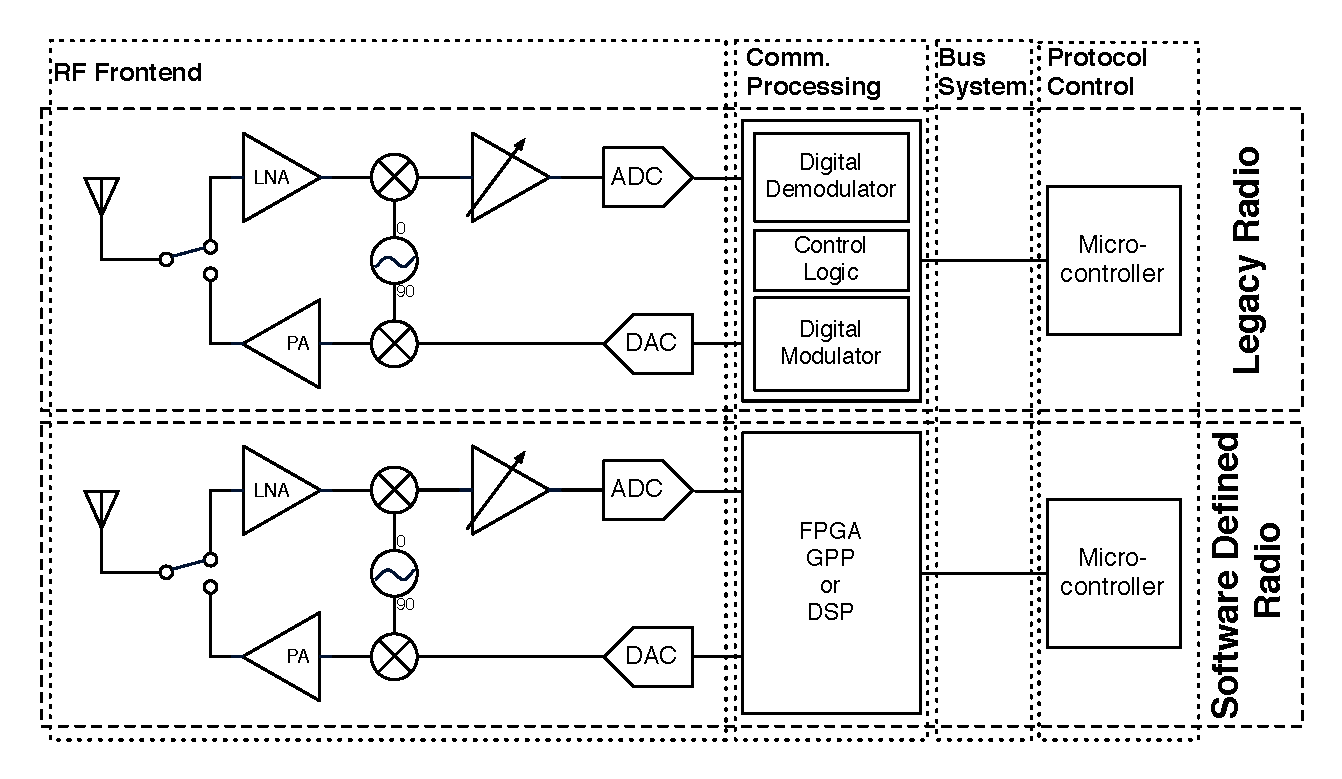
\includegraphics[width=0.98\columnwidth]{radio_vs_sdr}
\caption{Comparison of modern radio and a software defined radio. The main
difference is the fixed communication processing in a radio vs. the
reconfigurable processing possible in a SDR system.}
\label{fig:radio_vs_sdr}
\end{figure}
\end{comment}

\begin{table*}
\centering
\begin{threeparttable}
	\begin{tabular}{|l|c|c|c|c|c|c|c|} \hline
		\rowcolor[gray]{0}
		% header line
		\multicolumn{1}{|>{\columncolor[gray]{0}}c|}{\sc {\color{white} Platform}} &
		{\sc {\color{white} P$_{\text{Sleep}}$}} &
		{\sc {\color{white} P$_{\text{Active}}$}} &
		{\sc {\color{white} Size }}&
		{\sc {\color{white} Interconnect}}&
		{\sc {\color{white} Throughput}} &
		{\sc {\color{white} Price}} &
		% XXX: Usage -> adoption? Or some such metric is the idea behind this column
		{\sc {\color{white} Realization}}
		\\ \hline
		% SORA cost is totally estimated? No reference in the paper, but > PC cost..
		SORA {\small \cite{sora}}	 & -	& $>$100~W\tnote{c}	 & 36000~cm$^{3}$\tnote{c} & PCI-Express	& 16.7~Gb/s	& \$2000\tnote{c} & Research \\ \hline
		% KUAR power Pentium M min 5W, size COM Express 125 × 95 x (2 assumed) = 237.5, round 240, price: says "low cost" 3 times, but no price :(
		KUAR {\small \cite{kuar}}	 & -	& $>$5~W		 & 240~cm$^{3}$\tnote{f} &PCI-Express	& 2~Gb/s	& - & Research \\ \hline
		SODA {\small (180nm)~\cite{soda}} & -& \realtilde3~W & 26.6~mm$^{3}$\tnote{e}& DMA\tnote{a}	& 24~Mb/s\tnote{b} & -\tnote{d} & Simulated \\ \hline
		SODA {\small (90nm)~\cite{soda}} & -& \realtilde0.5~W & 6.7~mm$^{3}$\tnote{e}	& DMA\tnote{a}	& 24~Mb/s\tnote{b} & -\tnote{d} & Theoretical \\ \hline
		% WARP (numbers from energy wiki, where orig?), area 20 x 20 x >1, but we don't know it for sure so estimate conservative 2cm
		% Orig NRG num 10~15W, +30W / daughter card: 10~130W
		WARP~{\small \cite{warp-platform}} & -	& 10\realtilde130~W	 & 800~cm$^{3}$\tnote{f}	& Parallel MGTs\tnote{g}	& 24~Gb/s	& \$9750	 & Research \\ \hline
		%AirBlue Not really a platform
		% USRP 2, power 1.3-2.3A * 6V, area 22 x 16 x 5 cm
		% rate to/from host 50 MHz recv, 25 MHz xmit, 50/25 MSPS also
		% we'll go generous on the reported value
		USRP 2\tnote{c}~~{\small \cite{usrp:n200}}& -  & 7.9\realtilde13.8~W\tnote{c}	& 1760~cm$^{3}$\tnote{c} & Ethernet		& 1~Gb/s	& \$1700\tnote{c} & Commercial \\ \hline
		% E100, power 1.5-2.5A * 6V, area 22 x 16 x 5 cm
		% idle power is ~900mA * 6V = 5.5W
		% rate to/from host 4MHz, 4MSPS
% OMAP 3 GPMC Bus throughput: (we'll use best possible)
% http://e2e.ti.com/support/dsp/omap_applications_processors/f/42/t/35182.aspx#123019
		USRP E100~{\small \cite{usrp:e100}}& 5.5~W	& 9\realtilde15~W		 & 1760~cm$^{3}$		& OMAP 3 GPMC & 1.3~Gb/s	& \$1300	 & Commercial \\ \hline
		% uSDR, area 13 x 7 x 2
		\rowcolor[gray]{.9}
		\sdr	 & 0.32~W	& 1.4~W			 & 182~cm$^{3}$	& AMBA		& 1.4~Gb/s	& \$150\tnote{h}	 & Research \\ \hline
	\end{tabular}
	\begin{tablenotes}
		\small
		\item [a] Memory bus architecture not specified in~\cite{soda}.
		\item [b] Inferred minimum, may be faster.
		\item [c] Requires a companion PC. Not factored in power, portability, or cost for the USRP 1/2.
		\item [d] SODA is a custom chip that would likely have an extremely high die cost, but low per-unit cost.
		\item [e] Assumes $1mm$ thick.
		\item [f] Assumes $2cm$ thick.
		\item [g] ``Multi-Gigabit Transceiver'', an interconnect technology built into Xilinx FPGAs. Uses up to 8 parallel 3~Gb/s transceivers
		\item [h] Assumes 1,000 unit production run. See Table~\ref{tab:cost} for detailed breakdown.
	\end{tablenotes}
	\caption{A comparison of SDR platforms. The range in power comes from
boards whose power usage varies depending on the presence and type of daughter
card installed in the system. Where possible a measured idle / sleep power is
also shown.  For platforms that only list area we make reasonable assumptions
on height. \sdr is 10\% the cost of the next most expensive SDR platform, yet
provides parable speeds in the smallest non-IC package. It uses less power
than any realized hardware and nearly ties the previous best theoretical
hardware.}
	\label{tab:comparison}
\end{threeparttable}
\end{table*}
         % 1.5 pg
\section{Related Work}
\label{sec:related}

\begin{comment}
\begin{table*}
\centering
\begin{threeparttable}
	\begin{tabular}{|l|c|c|c|c|c|c|c|} \hline
		\rowcolor[gray]{0}
		% header line
		\multicolumn{1}{|>{\columncolor[gray]{0}}c|}{\sc {\color{white} Platform}} &
		{\sc {\color{white} Sleep}} &
		{\sc {\color{white} Power}} &
		{\sc {\color{white} Size }}&
		{\sc {\color{white} Interconnect}}&
		{\sc {\color{white} Throughput}} &
		{\sc {\color{white} Price}} &
		% XXX: Usage -> adoption? Or some such metric is the idea behind this column
		{\sc {\color{white} Realization}}
		\\ \hline
		% SORA cost is totally estimated? No reference in the paper, but > PC cost..
		SORA {\small \cite{sora}}	 & -	& $>$100~W\tnote{c}	 & 36000~cm$^{3}$\tnote{c} & PCI-Express	& 16.7~Gb/s	& \$2000\tnote{c} & Research \\ \hline
		% KUAR power Pentium M min 5W, size COM Express 125 × 95 x (2 assumed) = 237.5, round 240, price: says "low cost" 3 times, but no price :(
		KUAR {\small \cite{kuar}}	 & -	& $>$5~W		 & 240~cm$^{3}$\tnote{f} &PCI-Express	& 2~Gb/s	& - & Research \\ \hline
		SODA {\small (180nm)~\cite{soda}} & -& \realtilde3~W & 26.6~mm$^{3}$\tnote{e}& DMA\tnote{a}	& 24~Mb/s\tnote{b} & -\tnote{d} & Simulated \\ \hline
		SODA {\small (90nm)~\cite{soda}} & -& \realtilde0.5~W & 6.7~mm$^{3}$\tnote{e}	& DMA\tnote{a}	& 24~Mb/s\tnote{b} & -\tnote{d} & Theoretical \\ \hline
		% WARP (numbers from energy wiki, where orig?), area 20 x 20 x >1, but we don't know it for sure so estimate conservative 2cm
		% Orig NRG num 10~15W, +30W / daughter card: 10~130W
		WARP~{\small \cite{warp-platform}} & -	& 10\realtilde130~W	 & 800~cm$^{3}$\tnote{f}	& Parallel MGTs\tnote{g}	& 24~Gb/s	& \$9750	 & Research \\ \hline
		%AirBlue Not really a platform
		% USRP 2, power 1.3-2.3A * 6V, area 22 x 16 x 5 cm
		% rate to/from host 50 MHz recv, 25 MHz xmit, 50/25 MSPS also
		% we'll go generous on the reported value
		USRP 2\tnote{c}~~{\small \cite{usrp:n200}}& -  & 7.9\realtilde13.8~W\tnote{c}	& 1760~cm$^{3}$\tnote{c} & Ethernet		& 1~Gb/s	& \$1700\tnote{c} & Commercial \\ \hline
		% E100, power 1.5-2.5A * 6V, area 22 x 16 x 5 cm
		% idle power is ~900mA * 6V = 5.5W
		% rate to/from host 4MHz, 4MSPS
% OMAP 3 GPMC Bus throughput: (we'll use best possible)
% http://e2e.ti.com/support/dsp/omap_applications_processors/f/42/t/35182.aspx#123019
		USRP E100~{\small \cite{usrp:e100}}& 5.5~W	& 9\realtilde15~W		 & 1760~cm$^{3}$		& OMAP 3 GPMC & 1.3~Gb/s	& \$1300	 & Commercial \\ \hline
		% uSDR, area 13 x 7 x 2
		\rowcolor[gray]{.9}
		\sdr	 & 0.32~W	& 1.4~W			 & 182~cm$^{3}$	& AMBA		& 1.4~Gb/s	& \$150\tnote{h}	 & Research \\ \hline
	\end{tabular}
	\begin{tablenotes}
		\small
		\item [a] Memory bus architecture not specified in~\cite{soda}.
		\item [b] Inferred minimum, may be faster.
		\item [c] Requires a companion PC. Not factored in power, portability, or cost for the USRP 1/2.
		\item [d] SODA is a custom chip that would likely have an extremely high die cost, but low per-unit cost.
		\item [e] Assumes $1mm$ thick.
		\item [f] Assumes $2cm$ thick.
		\item [g] ``Multi-Gigabit Transceiver'', an interconnect technology built into Xilinx FPGAs. Uses up to 8 parallel 3~Gb/s transceivers
		\item [h] Assumes 1,000 unit production run. See Table~\ref{tab:cost} for detailed breakdown.
	\end{tablenotes}
	\caption{A comparison of SDR platforms. The range in power comes from
boards whose power usage varies depending on the presence and type of daughter
card installed in the system. Where possible a measured idle / sleep power is
also shown.  For platforms that only list area we make reasonable assumptions
on height. \sdr is 10\% the cost of the next most expensive SDR platform, yet
provides parable speeds in the smallest non-IC package. It uses less power
than any realized hardware and nearly ties the previous best theoretical
hardware.}
	\label{tab:comparison}
\end{threeparttable}
\end{table*}
\end{comment}

While there are a diverse array of SDR platforms~(\cite{warp-platform,
  soda, kuar, sora}), none of the current platforms are suitable for low
power radio research and development. In particular, \sdr optimizes
for power, price, and portability without appreciably sacrificing
flexibility or usability. A comparison to previous SDR platforms is
shown in Table~\ref{tab:comparison}.

\subsection{Throughput and Latency}
\label{sec:related-throughput}
% PCI-Express up to 25W max draw
As Schmid identifies in~\cite{schmid-latency}, a strongly limiting
factor for any SDR system is the available throughput and latency of
the interconnect between the ``hard'' and ``soft'' portions of the SDR
platform. As this latency defines the critical path for the control
loop, previous work places significant focus on minimizing it.

In developing SORA, the PCI-Express bus was selected for its bounded
latency and high throughput, at the cost
of its high power requirements and restricting the platform to the PC
form factor. This design affords SORA the support of a complete PC
operating system for multi-tasking and control, at the cost of
run-time adaptivity.
%
Ettus's USRP platform also relies on the PC operating system for much
of its command and control functionality, however it eschews the fixed
form-factor of the PCI-E bus, instead relying on more conventional
peripheral buses: USB or Ethernet. While these
buses do provide high throughput, Nychis et al. find their
latency to be highly variable, as high as
9000$\mu$s~\cite{cmu-mac-sdr}. For the development of low-power
protocols, such high and variable latency is untenable.

\begin{comment}
Ettus's USRP platform also relies on a controlling PC, however it trades
throughput for flexibility. The USRP is a run-time peripheral, utilizing
either USB (480~Mbits/s) or Ethernet (1~Gb/s) as a interconnect. The effective
rate, however, is limited by hardware components to 50~MHz receiving and 25~MHz
transmitting).  Nychis further shows in~\cite{cmu-mac-sdr} that the
variable latency of the USB and Ethernet interfaces further reduce the
effective throughput when reliable latency is required - a key component in
the development of low-power protocols. Ettus's embedded E100 platform suffers
from the same limitations, running a full Linux instance on the embedded
Gumstix platform to interface with the software radio over the same
channels~\cite{ettus}. % XXX: Did we ever prove this?
\end{comment}
%
% Okay SODA, I quit, I do not know how to reasonably compare your throughput /
% latency to any other platform. Intra-core speed is comparable to the
% processing power of the FPGA (when all cores are combined), inter-core
% throughput is probably best, but they don't report this at all...
Instead then, \sdr follows in the footsteps of SODA, tightly coupling
the hardware compute engine with an ARM Cortex-M3 core~\cite{soda}. Both systems
allow for low latency (0.46~$\mu$s) and high throughput
(172~MB/s). 
%(though OS's for the M3 do exist~\cite{coocox,etc})
Neither SODA nor \sdr use an operating system in the traditional
sense, however as a custom micro architecture, SODA goes even
further. It defines a slightly customized VLIW+SIMD ISA and sacrifices
traditional memory consistency semantics for performance. Users of
SODA then must carefully hand-tune their programs not only to optimize
performance, but to even run correctly. SODA is not a full-featured
SDR platform, rather an advanced DSP architecture. While this
microarchitectural compromise allows for better performance per watt,
\sdr has been realized in existing commodity hardware (as opposed to
just simulation), with a measured full system power draw only slightly
higher than SODA's theoretical optimized form, as
Table~\ref{tab:comparison} shows.
% also would like to say something here about \sdr not yet being at all
% optimized for power (gating, etc)

\subsection{Power}
\label{sec:related-power}
We first divide existing
SDR platforms into two broad categories: those reliant on a PC or
PC-architecture and those that are stand alone. Power and portability
are not a design consideration for these PC-platforms (SORA and USRP
2), thus it is unsurprising that \sdr, along with the other embedded
platforms, are orders of magnitude better in these metrics.

Of the remaining platforms, \sdr, KUAR, WARP, USRP E100, and SODA,
\sdr excels in power draw and is competitive in size with all except
the custom chip SODA. Both KUAR and the USRP E100 can be considered
``near-PC'' platforms that embed low-power, PC-like components in a
compact form factor.  KUAR does not explicitly report power numbers,
but builds a custom board driven by a Pentium~M whose most efficient
model draws 5~W~\cite{pentium-m}, which we use as a generously
conservative approximation for its power draw.  The USRP E100
datasheet reports 15~W load with RF daughtercard installed. In our
power measurements, shown in more detail in
Section~\ref{sec:eval}, we find an idle power draw of
5.5~W. The WARP base system draws about 10~W, but is capable of
supplying up to 30~W to each of four daughter cards, allowing for a
peak power draw of 130~W.

All of these previous systems have one thing in common: Their power usage is
reported in {\em watts}.  With \sdr, we deliver the first realized {\em
sub-watt} SDR platform.  This is a significant milestone. \sdr is the first
SDR platform capable of running for a full day on a pack of AA
batteries.
\begin{comment}
~\footnote{Extrapolating from~\cite{mote-power}, we consider four AA
batteries with average of 2500~mAh and a fully charged nominal voltage of
1.6V~. The minimum supply voltage to \sdr is 4~V, yielding 9.75~Wh of
usable power. This is enough energy for \sdr to run 7.5 hours at full power
or 30.5 hours in maximum sleep.}
\end{comment}
% Assuming a roughly linear scaling as # of batteries increases
% 2500mAh * 4.8V = 12Wh = 43200Ws
% 6.4-5.6V -- 31.25% of 43200 -> 13500
% 5.6-4.8V -- 27.10% of 43200 -> 11707.2
% 4.8-4.0V -- 22.90% of 43200 ->  9892.8
% Don't care after 4V.  Total -> 35100Ws (9.75Wh)

\subsection{Portability}
\label{sec:related-portability}
As we enter the era of {\em sub-watt} SDR platforms, we find that the
size, and in turn portability, of the SDR platform becomes a critical
design consideration. The current \sdr design is approximately four
times the size of popular research motes such as the Mica, TelosB, or
Tmote Sky, shown in Figure~\ref{fig:usdr}. We note that with the
removal of the external memory controller, \sdr's extra interfaces
(such as Ethernet), and a slightly more compact layout, the \sdr
platform could easily halve its size.

\subsection{Price}
Perhaps the greatest advantage of the \sdr system compared to previous
work is its extremely low cost -- an order of magnitude less expensive
than other SDR platform. The first large cost reduction comes from
building a standalone platform, rather than relying on a costly
support PC (SORA, USRP2) or the slightly less costly embedded PC-like
environment (KUAR, USRP E100). The next biggest saving comes from
eschewing the more traditional daughtercard based SDR approach,
instead opting to design a dedicated 2.4~MHz RF frontend. We note that
while the \sdr system lacks physical daughtercards, it does not
completely sacrifice modularity. Separate RF frontends can be
``dropped in'' to the schematic and used interchangeably. As evidence,
collaborators at other institutions
% Can we say this?
are already designing a new board with a 5~GHz frontend. We also find
considerable cost-savings by using fewer and less-powerful FPGAs than
the WARP platform. Despite the significantly lower processing power of
the \sdr platform, it is sufficiently capable of supporting an
802.15.4 radio, and building the radio on a significantly smaller
budget.

\begin{comment}
\subsection{Deployability}
Ultimately, \sdr contributes what we argue to be the first truly
{\em deployable} SDR platform. Previous platforms were tied to PCs
(SORA, USRP 2), tied to large power supplies (KUAR, WARP, USRP E100),
or existed only as simulations (SODA). Even resolving these issues,
all prior platforms were prohibitively expensive for any large scale
deployment. We estimate the cost per node of a 1,000 node \sdr
deployment to be only $\$150$, a full order of magnitude better than
the previous state of the art.
\end{comment}


       % 1.5 pg
%\clearpage
\section{Architecture}
\label{sec:arch}

This section presents the architecture and design decisions taken to
create the \sdr platform. At the heart of our design are three main
points: \emph{low-power}, \emph{small size}, and \emph{low cost}. We
relax the modular design of existing SDR systems to reduce size and
cost, while promoting the FPGA to a first class citizen.

As discussed previously, a fast interconnect is essential to achieve
low radio latencies which today's radio standards require. We have to
use a fast, but low-power interconnect between the FPGA and the
processing core to achieve this. One possibility is to use an external
memory interface existing on many low-power microcontrollers to
connect to the FPGA. While this allows for a flexible choice of
microcontroller and FPGA, it has the disadvantage of greater physical
space requirements, limited bandwidth due to a limited bus data width,
and potentially increased costs due to additional chip packaging
needs.

ARM provides several options both on the low-power computing core and
bus architecture front. All major FPGA vendors sell system-on-chip
packages that contain high-speed ARM cores integrated with
leading-edge FPGAs. The cores and the FPGA are most often connected
through the AMBA High-performance Bus (AHB). The AHB is a pipelined,
single clock-edge on-chip bus to connect peripherals, memories, and
cores on a system-on-chip and provides a bandwidth of up to
16~GBit/s. An even faster version of the AHB is the Advanced
eXtensible Interface (AXI) which is used in Xilinx's Zynq
reconfigurable SoC that marries a dual-core ARM Cortex-A9 with a
Xilinx FPGA in one package \cite{zynq}. Altera has a similar SoC
combining a dual-core ARM Cortex-A9 with their Arria V or Cyclone V
FPGA series. Altera's bus interface has a peak bandwidth of up to
100~GBit/s \cite{alteraSoC}. While these systems are very impressive
with respect to processing power and speed, their power draw is in the
multiple-Watts range, which is outside of our goal for a low-power,
battery-operated solution.

\begin{figure}[t]
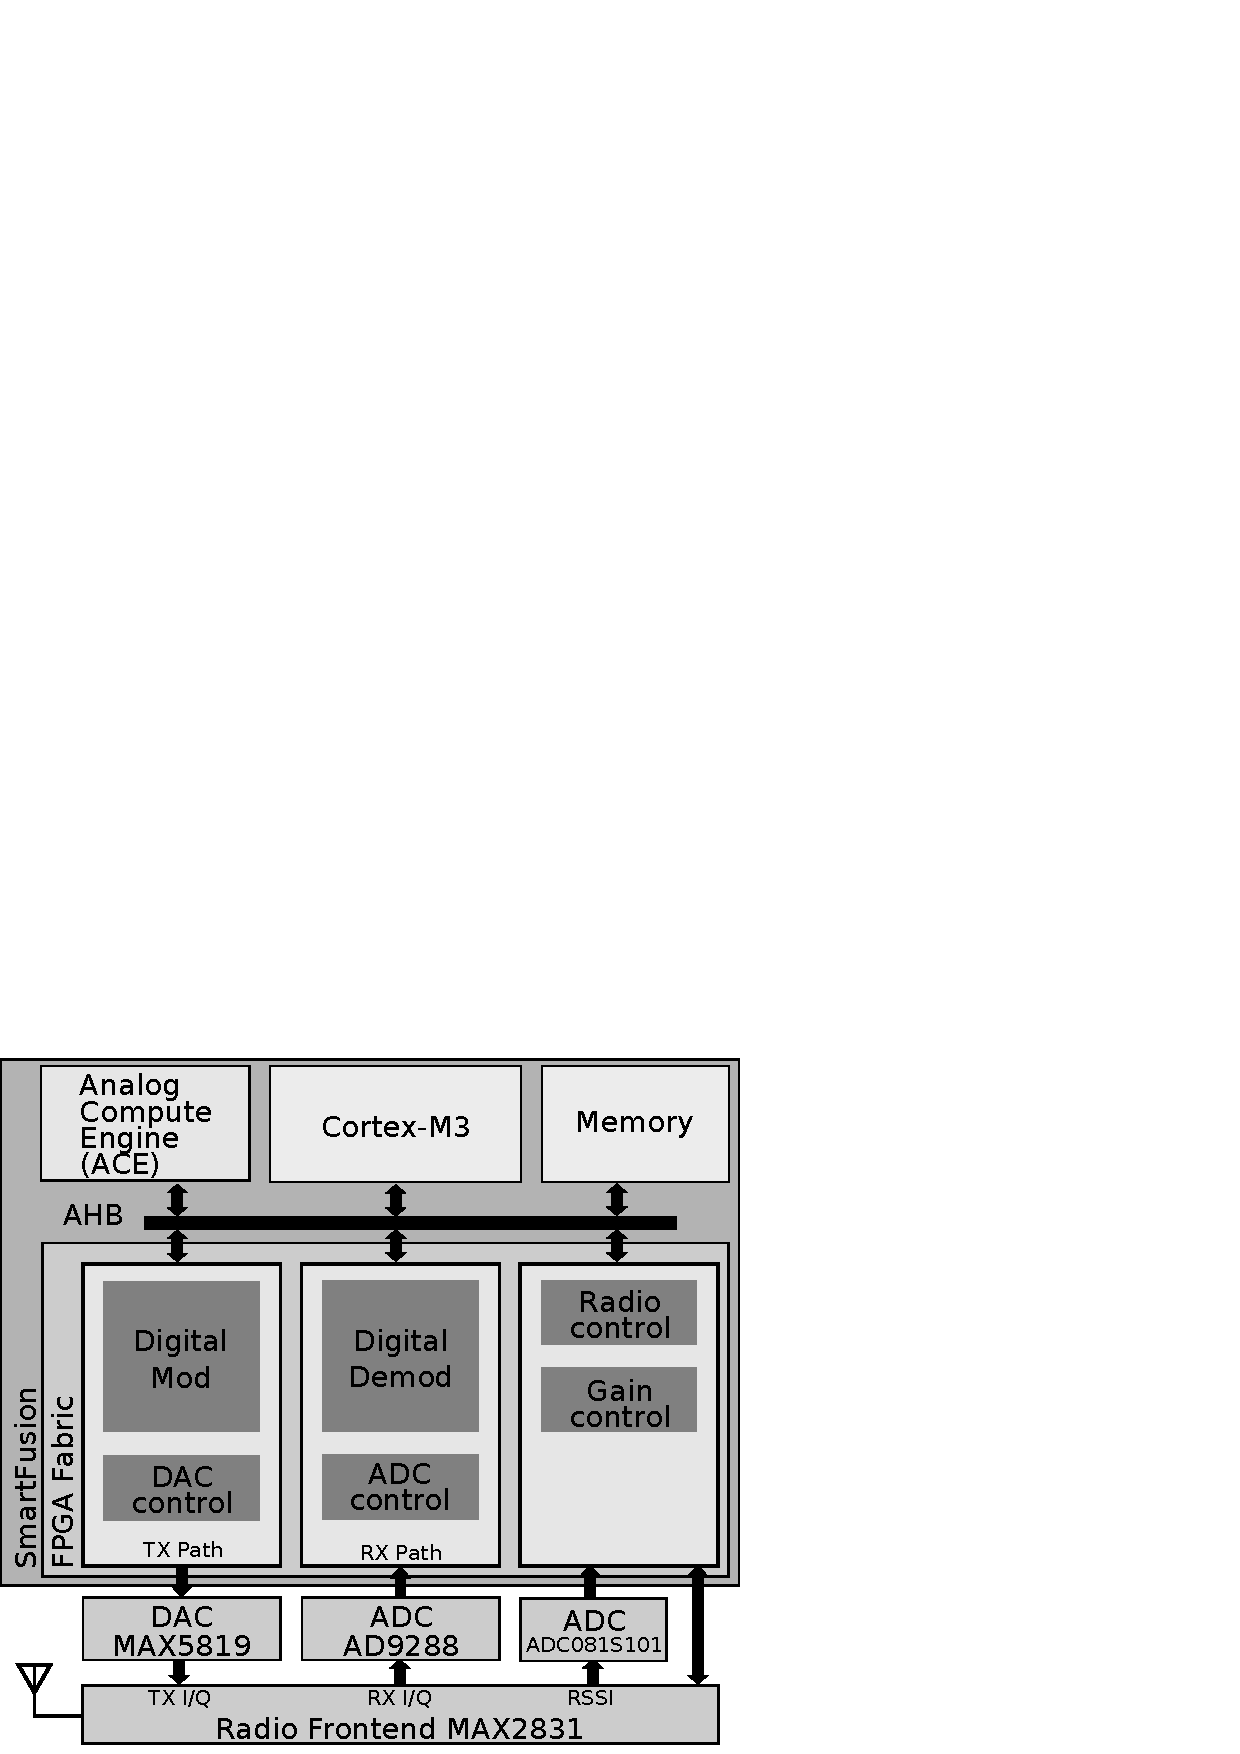
\includegraphics[width=0.98\columnwidth]{system_arch}
\caption{\sdr system architecture. The FPGA Fabric hosts the transmit,
receive, and radio control and is directly connected to the AMBA
High-performance Bus (AHB), together with the memory, analog compute engine
(ACE) and the ARM Cortex-M3 core. This rapid interface allows direct
memory-mapped access from the core to the SDR blocks. }
\label{fig:system_arch}
\end{figure}

\begin{figure}[th]
\includegraphics[width=0.98\columnwidth]{sdr_scale_tmote}
\caption{Picture of the \sdr platform. It measures 13~$\times$~7~cm and runs
for 7.5~hours without duty cycling from 4 AA batteries, allowing for the first
time true mobile SDR experiments. Shown for scaling is the TMote Sky. The
current \sdr is approximately four times the size of the Sky. Removing
extraneous inputs (Ethernet, etc) and debugging headers, \sdr is approximately
twice as large as the Sky.}
\label{fig:usdr}
\end{figure}

Microsemi, a vendor of flash-based FPGAs like the IGLOO series with
flash-freeze capabilities \cite{igloo} offers a third alternative in the
SmartFusion customizable System-on-Chip (cSoC). The SmartFusion contains an
ARM Cortex-M3 with a flash-based FPGA, connected through an AHB bus interface.
The flash-based FPGA brings the advantage of instant-on at power up, as the
configuration is stored in the FPGAs floating-gate memory. The AHB
interconnect allows a developer to write its own custom peripheral on the
FPGA, and access it through memory-mapped IO, as if it were a regular
peripheral. This allows for very fast and simple interaction between the
software and hardware side of the developed SDR code base, and a flexible
division between software-hardware boundary.

Beside the FPGA, the SmartFusion contains a rich set of standard
microcontroller peripherals (timers, serial bus interfaces, memories, etc) in
addition to an analog compute engine (ACE) with an ADC, DAC, and several
amplification and filtering options. By adding an RF radio frontend to the
ACE, the SmartFusion would be ready for SDR duties. However, at a maximum
speed of only $\sim$700~kS/s, the on-board ADC and DAC would limit us to low
data-rate communication.

We add an external high-speed ADC and DAC to the \sdr platform in order to
overcome the limits imposed by the ACE. Figure \ref{fig:system_arch} shows a
block diagram of the major components on the SmartFusion, as well as the
external ADC, DAC, and radio frontend chips. Figure \ref{fig:usdr} shows a
picture of the actual platform. The SmartFusion (U1) is the largest chip, located
at the center of the PCB. The ADC (U9) and DAC (U12) are located right of the
SmartFusion, and the RF frontend occupies the right-hand side of the board,
with the RF transceiver (U16) as the center piece.

\begin{comment}
\subsection{Chip Specifications}

This section covers specific chip details used on the \sdr platform.

We chose the largest SmartFusion currently available, the A2F500, which offers
512~kbyte of Flash and 64~kbyte of SRAM. The Cortex-M3 can run at up-to
100~MHz, and the FPGA provides 500,000 system gates and 24 dedicated RAM
blocks (at 4608 bits each), which is sufficient for many communication tasks or
complex custom logic.

The RF frontend is based on a Maxim MAX2831 RF transceiver chip operating in
the 2.4GHz ISM band. This RF transceiver combines all necessary RF blocks
reducing necessary external components and thus size and cost. This includes a
power amplifier (PA), RF-baseband converters, voltage controlled oscillator
(VCO), frequency synthesizer, and baseband control interface. The frequency
synthesizer supports step increments of 20Hz, and the digitally tuned
oscillator allows the MAX2831 to use a low-cost external crystal oscillator.
the MAX2831 has also a rich control interface using a serial peripheral
interface (SPI) as well as some dedicated I/O and analog lines for time-critical
operations, such as gain control and received signal strength indicator
(RSSI).

The external high-speed ADC and DAC are the Analog Devices AD9288~\cite{AD9288} and the Maxim
MAX5189~\cite{MAX5189}. The AD9288 is a high performance dual
channel analog to digital converter supporting up to 100~MS/s and draws less
than 90~mW per channel. The requirement for only a single power supply
simplifies the hardware design, and a power-down mode feature is necessary for its low-power
operation in duty-cycled applications. The MAX5189 is a low cost dual 8-bit
digital to analog converter, operating at up to 40~MS/s. In shutdown, the
MAX5189 draws only 5~$\mu$W.

In addition to the high performance parallel ADCs/DACs, a second serial ADC, the
ADC081S101~\cite{ADC081S101} is used to read the analog RSSI output of the RF transceiver
chip at up-to 1~MS/s. This information is available on the FPGA to implement
an automatic gain control algorithm for the low-noise amplifier of the RF
transceiver.
\end{comment}

%\subsection{Programming Environment}
%
%- Microsemi provides two software packages, Libero for the FPGA, and
%SoftConsole, an Eclipse based IDE, to program the Cortex-M3.
%- Libero offers an IP catalog
%- ??? what else ???

\subsection{Cost Breakdown}

Cost was a critical design aspect of the \sdr platform, necessary if one wants
to build larger testbeds and deployments of an SDR system. Table
\ref{tab:cost} shows the cost breakdown of the major \sdr components.  Even at
moderately small numbers (1k) the \sdr platform should cost less than \$150,
including assembly and PCB. 

\begin{table}[thb]\small
	\centering
	\begin{tabular}{|c|c|c|c|c|} \hline
	\rowcolor[gray]{0}
	  {\sc {\color{white} Desc}}
	& {\sc {\color{white} Part number}}
	& {\sc {\color{white} Size (mm)}}
	& {\sc {\color{white} Cost (1k)}}
	\\ \hline
	FPGA    & Microsemi A2F500M3G   & 17 x 17   & \$45 	\\ \hline
	Radio 	& Maxim MAX2831	        & 7 x 7     & \$4	\\ \hline
	ADC		& ADI	AD9288		    & 9 x 9     & \$4	\\ \hline
	DAC		& Maxim MAX5189 	    & 6 x 10    & \$5	\\ \hline
    Discretes &                     &           & \$34	\\ \hline
	PCB		& 6 layers      	    & 130 x 70  & \$25	\\ \hline
    Assembly &                      &           & \$20	\\ \hline\hline
	\rowcolor[gray]{.9}
    Total   &                       &           & \$137 \\ \hline
	\end{tabular}
	\caption{Cost breakdown of the \sdr platform.} 
	\label{tab:cost}
\end{table}

\begin{comment}
- High-level overview with block diagrams.
- AMBA bus memory map (ARM code, radio peripheral similar to SoCs with integrated RF)
-- Theoretic speed 16GBit/s. At 100 MHz bus speed, 3.2GBit/s more realistic (32-bit per clock cycle). But from current Section 4.2, we only get 37 MBit/s?
    o 48 MHz, 1 byte transfers, 4 cycles per transfer (+ transfer to RAM + start PDMA to done signal)
- How do we implement basic comm blocks (software vs. hw, correlators, filters, etc)
 -- (not building blocks that are available, rather how do you use this platform to build something)
- What kind of performance can we expect from it?
- What is the maximum bandwidth achievable (impulse response)
- How does it fit our defined requirements from intro?
-- Power Measurements of basic platform
-- Performance of blocks
\end{comment}
          % 2.5 pg
%\section{Applications}
\label{sec:applications}

\begin{table}[b]
\centering
\begin{threeparttable}
\begin{tabularx}{\columnwidth}{|X|X|X|}
    \rowcolor[gray]{0}
   {\sc {\color{white} Component}}
 & {\sc {\color{white} Area}}
 & {\sc {\color{white} Max Freq}}
\\\hline
TX & 20\% & 100 MHz \\\hline
RX & 72\%\tnote{a} & 80 MHz\tnote{b} \\\hline
\end{tabularx}
\begin{tablenotes}
	\small
	\item [a] Area optimized for minimum required frequency of 16~MHz.
	\item [b] Speed optimized increases area to 78\%.
\end{tablenotes}
\caption{FPGA size and corresponding maximum frequency. The area with
respect to the 500k gate SmartFusion A2F500. The transmitter is limited by
80~MHz DAC, while the receiver is FPGA limited.}
\label{tab:area}
\end{threeparttable}
\end{table} 
This section presents the viability of using the \sdr platform to communicate
with standards compliant low-power radios. We decided to implement IEEE
802.15.4, a non-trivial physical communication specification used in many
short-range, low-power radios. 

The short-range low-power wireless standard IEEE 802.15.4 describes the
physical layer and frame structure, leaving the higher layers up to the
developer to design. IEEE 802.15.4 uses spread spectrum technology to increase
its resilience towards channel noise. Every 4-bit data sequence gets mapped to
a 32-bit long chip sequence. This chip sequence is then modulated as an
offset quadrature phase-shift keying (O-QPSK) signal with half-sine pulses. The sixteen
32-bit chip sequences are chosen such that their autocorrelation is minimized.
This allows a receiver to compare incoming chip sequences to one of the sixteen
existing sequences, allowing for errors within the received
sequence, but resulting in a successful sequence detection with high
probability.

IEEE 802.15.4 is a packet-based standard. Each packet, or frame, consists of a
pre-defined sequence. At first, every packet starts with a preamble of four
bytes of 0x00. This is followed by the Start of Frame Delimiter (SFD) byte
0xA7. The preamble is used to condition a radio and detect an incoming packet,
while the SFD signals the beginning of the data. The first data byte has to be
the length of the rest of the packet. Following the length byte comes the
Frame Control Field (FCF). The FCF is a two byte value indicating different
properties of the message, such as addressing mode (length of addresses used),
is an acknowledgment requested, etc. Following the FCF comes a one byte
sequence number (Data Sequence Number, DSN) followed by the address
information. For data integrity, IEEE 802.15.4 uses a two byte long Cyclic Redundancy Check
(CRC). The CRC is added to the very end of a message.

Figure \ref{fig:system_arch} shows the general \sdr architecture. For our IEEE
802.15.4 implementation, we implemented a transmitter with O-QPSK modulator
representing the transmit path. For the receiver we exploit the fact that
O-QPSK with half-sine pulse shapes is equivalent to minimum shift keying
(MSK), and thus we use an FM demodulator. The following sections go into
details of the specific implementations. To exemplify the potential of the
\sdr platform, we describe in Section \ref{subsec:enhance} enhancements we
performed that usually are not found on commercial radios, but support recent
advances in wireless protocol designs.

%Different SDR platforms target different design spaces, ranging from
%full-software inmplementation on a general purpose processor like in GNU
%Radio or MSR's SORA, to radios with highly reconfigurable hardware like the
%WARP. \sdr explores the architecture trade-off between hardware and software
%to build a SDR platform which is well suited for mobile, low-power
%applications. Compared to GNU Radio or MSR's SORA which use a commodity PC as
%baseband processor, \sdr has limited computing resources available. Therefore,
%\sdr implements the basic radio functions in the reconfigurable hardware.
%While this puts a bigger burden on the developer, as the radio blocks have to
%be implemented in a Hardware Description Language (HDL), it makes the system
%resemble regular radios, as the interface between software and hardware
%are memory-mapped registers. 

\subsection{Transmitter}

We implemented the full transceiver chain as a memory-mapped peripheral on the
FPGA. This reduces the burden and complexity of the software. To send out a
message, the core transfers the packet from memory into a transmit fifo (see
Figure \ref{fig:transmitting_chain}). The processor can start the transmission
before the full packet is uploaded by sending a transmit command to the
peripheral. The peripheral starts encoding the packet, starting with the
preamble, SFD, and FCF, before adding the bytes from the transmit fifo. The
bytes go through several encoding steps, translating from half-bytes (4-bit) to
chip sequence (32-bit), and finally getting mapped to an O-QPSK signal with
half-sine pulse shapes on the in-phase and quadrature band. All these
translations are done by using lookup tables, simplifying the implementation
while providing high-speed processing.

The transmit fifo shares the transmit chain with two other fifos for
automatic acknowledgment generation and rapid message forwarding. An access
control logic grants permission to a fifo if the fifo has data to transmit,
and the transmit chain is currently empty. Section \ref{subsec:ack} and
\ref{subsec:forward} will go into more details on these two fifos.

\begin{figure}[bht]
\centering
\includegraphics[width=0.98\columnwidth]{transmitting_arch}
\caption{IEEE 802.15.4 transmitter implementation. Three input FIFOs feed the
modulator implemented as lookup tables for byte to chip, and chip to half-sine
pulse mapping. This provides a compact and simple O-QPSK implementation with
support of automatic ACK generation and fast packet forwarding mechanisms.}
\label{fig:transmitting_chain}
\end{figure}

\subsection{Receiver}
 
\begin{figure}[h!]
\centering
\includegraphics[width=0.98\columnwidth]{receiving_arch}
\caption{IEEE 802.15.4 receiver implementation. Our implementation exploits
the fact that O-QPSK modulation can be decoded as MSK with adaptation of the
chip sequences. This simplifies the decoder implementation.}
\label{fig:receiving_arch}
\end{figure}

The implemented receiver chain (compare Figure \ref{fig:receiving_arch} resembles
the GNU Radio IEEE 802.15.4 receiver implementation described in
\cite{Schmid:802.15.4}. It exploits the fact that an O-QPSK modulated signal
with half-sine pulse shapes is equivalent to a minimum-shift keying (MSK)
signal, and thus a simpler frequency shift keying (FSK) demodulator can be
used to extract the chip sequence from the data stream \cite{cmos:rfic}. The
FSK-demodulator uses the in-phase and quadrature components coming from the RF
chip at 16~MS/s and produces an amplitude modulated (AM) signal, where the amplitude
corresponds to the frequency of the incoming signal. A matched filter
integrates the AM signal. The filter is sampled at the chip-frequency of
2~MS/s, indicating a logic 1 or 0. A preamble detection mechanism searches for
a 0x00 (a chip sequence of 64 bits) to identify incoming
packets. It also performs clock synchronization by occasionally adjusting the matched
filter. The receiver then calculates the Hamming distance $D$ between detected
symbols and the known chip sequences. The decoded symbol is the
index of the sequence that has the minimum distance $D$ from the sampled
sequence. The smaller the distance $D$ from a known chip sequence, the higher
the probability for a correct decoding. Once the symbol is decoded, the
receiver stores the decoded symbol in a \emph{RX fifo} and performs the frame
filtering. Various interrupts (detection of the start of frame delimiter SFD,
Length, Packet completed etc) are generated during the frame filtering,
informing the processor of the different events happening in the decoder.
These interrupts are crucial for timely processing inside the software
implementation of a MAC protocol.
Once a packet is fully received (e.g. when the processor receives the Packet Completed 
interrupt), the processor copies the packet from the RX fifo using a DMA
transfer into RAM for further processing.

\subsection{Radio and Automatic Gain Control}

A flexible SDR system needs fast and extensive control over the radio frontend
in order to be agile and adapt to a changing RF environment. The MAX2831
provides a 3-wire SPI interface for configuration, a 7~bit parallel bus for only gain
control, and an analog output providing the received signal strength. An
additional I/O line switches the frontend from receive to transmit, i.e., the
chip can not be used for full-duplex radio communication.

We offload as much of the radio control into the FPGA as possible. This 
simplifies the software to memory-mapped operations instead of dealing with a
stand alone SPI interface and incurring potential software interrupt
latencies. In addition, it speeds up the control loop and allows us to send
commands to the radio within $\mu$s. For example, the MAX2831 does not provide an
Automatic Gain Controller (AGC) built into the package. Thus, the FPGA has to
measure the RSSI, and adjust the radio gain through the SPI 
interface. The AGC loop tunes the gain setting within 5~$\mu$s without having
to involve the processor. This high speed AGC keeps tuning the gain setting to
prevent abrupt changes in signal strength and maintains a constant signal
amplitude.

\subsection{Hardware ACK Generation}\label{subsec:ack}

Many wireless protocols rely on acknowledgment messages (ACK) to ensure the
reliability of a transmission. According to IEEE 802.15.4, if a receiver
received a packet requesting an ACK, it has to generate an ACK frame and respond
to the transmitter in precisely 192 $\mu$s. Meeting this timing constraint can
be difficult for an SDR platform if they rely on the processor to software
decode the signal. Pure software decoding is favorable from a software
engineering's perspective, as more resources and code libraries are available.
In addition, the code can be written in a higher level language, such as C/C++
or Python. However, software decoding platforms must have enough computing
resources and low-latency interfaces between the processor and radio to meet
the stringent timing constraints. In most SDR systems, the interface between
the processor and the radio frontend is considered the data bottleneck.

Meeting those strict timing constraints has become a challenge to SDR
platforms. Nychis et al. characterize in \cite{2009.Nychis.nsdi} various
latencies from the Linux kernel to the Universal Software Radio Peripheral's
FPGA. Their results showed that it can take up to 9,000~$\mu$s with a mean
latency of 612~$\mu$s to get data from the Linux kernel to the USRP. Because
of this nondeterministic latency, the USRP is ill-suited for any
timing-constraint communication protocol. Nychis proposed several basic RF
blocks that if implemented close to the radio, can alleviate this problem.
However, it makes the system architecture significantly more complex to use as
this partition must be carefully planned.

MSR's SORA solves the interface issue by using a high bandwidth and
low-latency PCI-E interface, which achieves 360~ns one-way delay.
Additionally, a powerful multi-core processor with dedicated processing cores
allows real-time decoding and fast replies.

In contrast, the \sdr design uses hardware decoding, i.e., demodulation and
frame filtering are all performed in the FPGA. This drastically reduces
decoding latency and allows \sdr to quickly respond to incoming packets. In
\sdr, the ACK frame generation is also implemented in hardware. The ACK
generation block pre-stores preambles and SFD in a small 11-byte ACK fifo. The
only missing parts of the ACK are the data sequence number (DSN) and
corresponding FCS. If the incoming packet passes the CRC check, the hardware
copies the packet's DSN into the ACK fifo. At the same time, the ACK generator
block calculates the corresponding FCS and initiates a countdown for precise
timing. In our IEEE 802.15.4 implementation, the receiver calculates the CRC
and FCS within 12~$\mu$s, leaving 180~$\mu$s of slack for timing requirement.

\subsection{Radio Enhancements}
\label{subsec:enhance}

The receiver, transmitter, and hardware acknowledgment implementations are
everything needed to fully interact with commercially available IEEE 802.15.4
radios. The following sections describe enhancements to support more advanced
MAC features that are not always found in currently available radios. This
highlights the strength of \sdr to test and validate new radio architectures
that jointly optimize low-power MAC protocols.

\subsubsection{Multiple Address Recognition}

The most important decision a low-power MAC protocol makes is to stay awake or
go back to sleep if channel activity has been detected. Recent advances in
low-power MAC protocols showed that receiver initiated protocols have an
advantage over low-power listening types of protocols as they are more robust
against interfering noise \cite{2010.amac}. In a receiver initiated MAC
protocol, nodes that want to receive packets transmit a short probe. Nodes
that have packets to transmit buffer them locally until they hear a beacon
from the intended receiver. Once they decoded a beacon, the nodes acknowledge
it and start transmitting the data in the next packet. A-MAC \cite{2010.amac}
demonstrated that this can be done in a very efficient way, even if multiple
nodes try to send data to the same receiver. A-MAC exploits the fact that
acknowledgment messages will interfere constructively at the receiver. This
allows the receiver to make the crucial decision to stay awake, even if the
first data packet of the multiple transmitters collides, at which point a
back-off mechanism must resolve the conflict.

\begin{figure}[bht]
\centering
\includegraphics[width=0.98\columnwidth]{addr_recog_blk}
\caption{Packet reception and response in \sdr. This diagram shows the
paritioning of responsibilities between the hardware and software portions of
\sdr. The decision to support multiple address recognition requires software
support of the reception/response loop to keep hardware area costs reasonable.
In this tightly coupled model, the software controller takes advantage of the
hardware accelerated acknowledgments to meet the stringent latency
requirements of the 802.15.4 acknowledgment frame.}
\label{fig:addr_blk}
\end{figure}

Dutta et al. found in \cite{2010.amac} that a limiting factor of implementing
A-MAC is the address recognition mechanism of the radio. Hardware
acknowledgments can only be generated for ones own address. Thus, A-MAC
reprogrammed it's own address to the intended receiver's beacon address
(receiver's address with the MSB bit set) waiting for the beacon. This
introduced several problems and limits the protocol.
% Should we indicate at all what problems specifically this causes?

We implemented a multiple address recognition mechanism in \sdr. According to
the IEEE 802.15.4 standard, the address field can be as long as 8 bytes. This
leads to a design trade-off between implementing this functionality in
software or hardware by trading latency for FPGA area. We decided to have a
slight latency increase, and implemented a multiple address recognition
algorithm on the processor that can detect up to 8 addresses. However, this
latency increase does not impact the performance of the protocol, as \sdr can
read out the address faster from the receive fifo than the time it has to wait
to reply with an ACK. In addition, the multiple address recognition algorithm
takes advantage of the hardware acknowledgment mechanism preparing an ACK
while receiving the incoming packet. All the algorithm has to do is send a
signal to the peripheral letting it know to acknowledge this message.  Figure
\ref{fig:addr_blk} shows the state diagram of the algorithm and how the
hardware and software interact with each other. This demonstrates the
flexibility of the platform, allowing certain protocol functionalities that
are time critical to be done in hardware only (e.g.  hardware acknowledgments
generation) while others are implemented in software.


\subsubsection{Packet Forwarding}\label{subsec:forward}

\begin{figure}[ht]
\centering
\includegraphics[width=0.98\columnwidth]{fwd_blk}
\caption{Detailed packet forwarding state diagram. This is a more detailed
version of the packet forwarding mechanism shown on Figure \ref{fig:addr_blk}.
Packets are stored in an incoming FIFO, automatically incrementing the Relay
Count field and CRC as necessary. When a packet completes, it is automatically
forwarded if requested and its count is below the relay threashold.}
\label{fig:fwd_blk}
\end{figure}

Two basic services in wireless sensor networks are time synchronization and
flooding. The broadcast storm~\cite{syn:broadcast} is a common problem
flooding algorithms have to take care of, as retransmission of regular
broadcasts can amplify itself, and thus overload the network. Ferrari et al.
proposed {\em Glossy}~\cite{ferrari:efficient}, a fast flooding and time
synchronization mechanism. Glossy exploits the fact that in IEEE 802.15.4, if
multiple identical packets arrive within 0.5~$\mu$s at a receiver, they
collide constructively, and the receiver can successfully decode the message
with high probability. To achieve this, Glossy nodes forward a received packet
during a precise time slot and increment a relay counter in the packet.
Packets with identical relay counts will be transmitted at the same time, at
all nodes. Therefore, the packets will constructively interfere at the
receivers. The relay counter limits the maximum hop count of the packet,
making sure that packets don't live forever within the network. Glossy uses a
fragile software technique to guaranty software latencies. They have to
disable all interrupts and add no-operation (NOP) commands to adjust the
latencies during a Glossy transfer. Although the wireless links are lossy,
Glossy demonstrates 99.9999\% flooding reliability in a 10 hop deep network.

\"{O}sterlind et al. proposed in \cite{zero_copy} a zero-copy mechanism to
improve the throughput of multi-hop wireless sensor networks. He observes that
the critical path of zero-copy is the interface between radio and processor.
The packet forwarding is done by downloading the packet from the radio to the
processor, and uploading it back into the radio. Instead of
downloading and then uploading the same packet, it would be advantageous if
the radio stored the received packet and were able to immediately retransmit
it out. This method improves the total throughput to 97\% of the theoretical
upper bound.

We decided to implement a fast packet forwarding mechanism in the FPGA of the
\sdr platform. We use the data sequence number (DSN) as a relay counter.
Figure \ref{fig:fwd_blk} shows the state diagram. During reception of a
packet, the receiver stores the data in two different fifos, the receiver and
forwarding fifos. However, the two fifos store slightly different information
in the DSN and frame control sequence (FCS). The DSN gets automatically
incremented by 1, and the FCS is updated accordingly.

Using this mechanism, \sdr forwards a packet without interacting with the
software at all. This removes the critical path identified by \"{O}sterlind
and allows the retransmit to happen in less than 20~$\mu$s. This forwarding
also solves the fragile Glossy software implementation as no interrupts have
to be disabled on the software side, nor do we have to add any NOPs. In
addition, the forwarding can be precisely controlled, changing the latency to
any arbitrary, but fixed, delay (e.g. to 192~$\mu$s which would correspond to
the ACK turn around time). This would allow backward compatibility with some
existing commercial radios that have forwarding capabilities (e.g. the TI
CC2520), but have a transmit to receive turn around time of 192~$\mu$s as
specified by the IEEE 802.15.4 standard.

%- What can we do with this SDR platform?
%- E.g. IEEE 802.15.4 implementation. Why is that even interesting?
%  -- standards compliant == compliant with commercial radios
%  -- we built two radios (one basic FSK, one standards compliant)
%- Explain \& block diagram of TX and RX chain
%- Address Recognition
%- ACK generation
%- Message Forwarding
  % 2.5 pg
\section{Evaluation}
\label{sec:eval}

We evaluate \sdr on its merits as a low-power SDR platform. Specifically, we
focus on its power consumption, latency, and hardware flexibility. We further
examine the performance of the \sdr system in the exploration of the low-power
802.15.4 MAC protocol.

\vfill\eject

\subsection{Platform Micro-Benchmarks}
Designing a low-power system requires building from the ground up with
low-power components. In traditional software radio designs, one of the
largest power sinks is the FPGA. The recent influx of flash-based FPGAs open
the door to low power design. In Table~\ref{tab:fpga_static_current} we
compare the static power draw of the flash-based SmartFusion to the SRAM-based
Xilinx Spartan~3-2000 used in the USRP 2. The superior FPGA core power
efficiency of the flash-based FPGA is a direct consequence of the technology.
Freed of the requirement to continually refresh the logic cells, the flash
FPGA consumes very little static power. As a young technology, we expect these
innovations in static power for flash-based FPGAs to improve rapidly, as
evidenced by the Microsemi IGLOO series, whose Flash*Freeze technology lowers
the FPGA static power draw as far as 2~uW~\cite{igloo}.

In addition to the impact on static power usage, flash-based FPGAs also excel
during cold-boot. For an FPGA to be useful, it must at some point be
configured. In the case of SRAM-based FPGAs, this configuration must occur at
every boot, as the configuration of the FPGA is lost when power is no longer
supplied. This configuration period introduces a non-trivial delay for the
FPGA wake-up process as well as consuming a relatively large amount of power.
Most importantly, the latency imposed by the configuration window inhibits
effective duty-cycling of the FPGA. In Figure~\ref{fig:coldboot}, we compare
the cold boot times of the SRAM-based USRP 2 (\ref{fig:usrp_coldboot}) to the
\sdr (\ref{fig:usdr_coldboot}). After a system in-rush current spike of
1.8~A, the USRP 2 averages a 700~mA current draw for 1.964~s while it
configures its FPGA. This long configuration process and high current
consumption consume 9.56~J of energy, a cost that must be paid every time the
FPGA is power cycled.

\begin{table}
	\centering
	\begin{tabular}{|c|c|c|}
		\hline
		\rowcolor[gray]{0}
		 % first column blank
		 & {\sc {\color{white} SmartFusion}}
		 & {\sc {\color{white} Spartan}} \\ 
		\rowcolor[gray]{0}
		  {\sc {\color{white} voltage rail}}
		& {\sc {\color{white} static current}}
		& {\sc {\color{white} static current}} \\ \hline
		3.3V (IOs )	& 85.6 mA 	& 79 mA \\ \hline
		2.5V (Aux) 	& n/a		& 88 mA \\ \hline
		1.5V (Core)	& 7.76 mA 	& n/a   \\ \hline
		1.2V (Core)	& n/a		& 80 mA \\ \hline
		\rowcolor[gray]{.9}
		Total Power	& 294 mW	& 578 mW \\ \hline
	\end{tabular}
    \caption{Static current at each supply rail for the SmartFusion and
In contrast, \sdr has no current spike on bootup and an average current
consumption of under 100~mA. To measure time to first useful instruction, we
wrote a simple program that simply toggles an IO line, indicating the
processor is ready to start executing. We measured the time from power
application until the IO asserts. The \sdr requires 259~ms to boot the system,
consuming only 0.101~J. Even the latency of \sdr is not ideal for a rapid
duty cycled system, which would ideally be in the {\em microsecond} range as
opposed to {\em milliseconds}. \sdr is remains significantly better than the
USRP 2's {\em seconds} to boot: $7.6\times$ faster in terms of latency and
$94.7\times$ lower in terms of energy consumption.
platforms.}
	\label{tab:fpga_static_current}
\end{table}

\begin{figure*}[t]
	\centering
    \subfigure[USRP2 Cold Boot]{
        \includegraphics[width=0.45\textwidth]{usrp_coldboot/usrp_coldboot}
        \label{fig:usrp_coldboot}
    }
    \subfigure[\sdr Cold Boot]{
        \includegraphics[width=0.45\textwidth]{usdr_coldboot/usdr_coldboot}
        \label{fig:usdr_coldboot}
    }
    \caption{USRP2 and \sdr cold boot comparison. Both systems power on at
{\em 0~s}. As expected, the USRP2 \subref{fig:usrp_coldboot} has a current
spike of 1.8~A, and exhibits an average current draw of 700~mA at 6~V. It
takes 1.96~s to load the firmware from an external SD card, resulting in
9.56~Joules of energy consumption during cold boot. In contrast, the
flash-based \sdr doesn't have an in-rush current and the average current is
less than 100~mA at 3.3~V. Moreover, \sdr requires 259~ms to boot the system,
resulting in only 0.101~Joules of energy consumption. \sdr is 7.6$\times$
faster and uses 100$\times$ less energy than the USRP2 to start-up.}
\label{fig:coldboot}
\end{figure*}

Given that the 259~ms boot time is too highly latent to support aggressive
duty-cycling, \sdr also presents a sleep mode as a median option between
system full on and full off. Unfortunately, the SmartFusion chip is only
capable of sleeping the M3 core (via WFI\footnote{WFI: Wait For Interrupt, and
ARM instruction that places the core in a lower power sleep state until
interrupted. The contents of registers are preserved but the rest of the core
is power gated}). Fully sleeping the FPGA would require technology similar to
the Flash*Freeze mode from the Microsemi IGLOO line of low-power FPGAs.
Unfortunately these FPGAs do not yet support the tight integration with a hard
CPU and are currently unsuitable for the \sdr platform. Until technology
similar to Flash*Freeze comes to the SmartFusion, \sdr is still capable of
lowering the FPGA power via frequency scaling. In \sdr's frequency scaling
mode we turn off the external crystal oscillator and used the FPGA's internal
RC network instead. The frequency of the RC network is reduced to 6.5\% of
the original frequency (to 3.125~MHz). We additionally turned off the PLL and
bypassed two other clock sources for FPGA logic to further reduce the system
current. Table~\ref{tab:sdr_wfi_duty_cycle} examines the impact of these power
saving efforts. Simply placing the processor in WFI state and power gating all
external components reduces system power consumption to 108~mA with only
34~$\mu$s of wakeup latency. Introducing FPGA frequency scaling reduces
system power further to 67~mA, but imposes a 3.01~ms latency to turn on the
crystal oscillator and stabilize the PLL until the processor can be woken.

\begin{table}[h]
	\centering
	\begin{tabular}{ | c | c | c | }
		\hline
		\rowcolor[gray]{0}
		  {\sc {\color{white} Frequency}}
		& {\sc {\color{white} Wake-up}}
		& {\sc {\color{white} System}}
		\\
		\rowcolor[gray]{0}
		  {\sc {\color{white} Scaling}}
		& {\sc {\color{white} Latency}}
		& {\sc {\color{white} Power}}
		\\ \hline
% 108mA * 4.8 , 67 * 4.8
		off	& 34 $\mu$s	& 518 mW \\	\hline
		on	& 3.01 ms	& 322 mW \\	\hline
	\end{tabular}
    \caption{Sleep power and latency trade-off.  Without frequency scaling,
\sdr draws 108~mA while Waiting For an Interrupt {\em WFI}. It wakes-up from
this state in only 34$\mu$s. With frequency scaling, \sdr saves 38\% in power
while taking 89$\times$ longer to wake up.}
	\label{tab:sdr_wfi_duty_cycle}
\end{table}

Spartan~3-2000. The Spartan is a more traditional SRAM-based FGPA whereas the
SmartFusion is a flash-based design. Measurements are taken after both devices
have been configured and allowed to settle. We observe similar static current
at the IO buffers, but significant differences at the core supply. The
SmartFusion current is 10$\times$ less than the Spartan. As a consequence, the
SmartFusion requires approximately half as much static power as the Spartan,
making flash-based FPGAs a much better desgin decision for low-power

We finally compare \sdr to the USRP E100, USRP's ``embedded'' series. The E100
is built on the GumStix platform, a small ARM-based PC-like device. The
advantage of the E100 is it requires no controlling computer, rather it is
built in to the system. As a consequence, however, we find in
Figure~\ref{fig:usrp_e100} that the E100 actually has greater power draw that
it's PC-encumbered counterpart.


\begin{comment}
\begin{table}
	\centering
	\begin{tabular}{|c|c|c|} \hline
		\rowcolor[gray]{0}
		  {\sc {\color{white} AGC mode}}
		& {\sc {\color{white} Average ARR}}
		& {\sc {\color{white} Std}}
		\\ \hline
		SFD-latch 	& 97.27\% 	    & 0.211\%	\\ \hline
		Continuous	& 98.20\%	    & 0.065\%	\\ \hline
	\end{tabular}
    \caption{Acknowledgment reception rate (ARR) for two constructively
interfering transmitters with respect to different AGC modes. We transmitted
10,000 ACKs per transmitter per experiment and repeated each experiment 5
times. A continuous AGC performs slightly better due to the small carrier
frequency separation of the transmitting nodes.}
	\label{tab:ARR_versus_agc_mode}
\end{table}
\end{comment}


\begin{figure}[h]
	\centering
	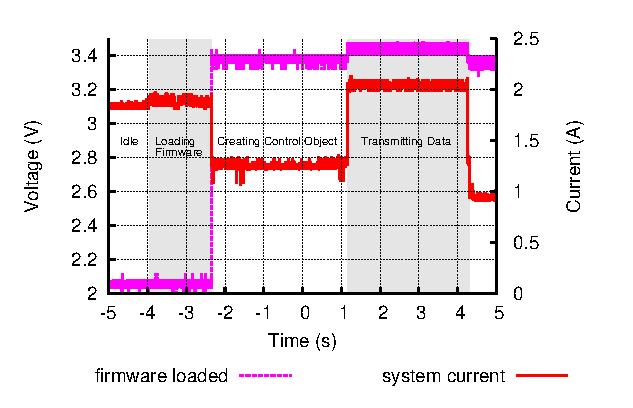
\includegraphics[width=0.98\columnwidth]{usrp_e100_run/usrp_e100_run}
	\caption{USRP E100 power profile. E100 runs a full embedded Linux
platform, making cold-boot an untenable comparison. Rather we show the timing
from an idle, booted system to load a firmware image (configure the FPGA) and
send the data.  The firmware loaded signal is recorded from a firmware loaded
pin. After configuration, the system idle power drops to
just under 1~A at 6~V.}
	\label{fig:usrp_e100}
\end{figure}

\begin{comment}
\subsection{Application Micro-Benchmarks}
To evaluate the \sdr system as a whole, we first compare the raw radio
performance against a current low-power radio: the TI CC2420. We then explore
the implementation of two recently proposed low-power protocols: A-MAC and
Glossy.

\subsubsection{Comparison with a CC2420}

\begin{figure}
	\centering
	\includegraphics[width=0.98\columnwidth]{R_inputPWR/R_inputPWR}
	\caption{Received signal strength vs. packet error rate (PER) of \sdr. If
the received signal strength is $>$~-90~dBm, then we have a PER of $<$~1\%. As a
comparison, the TI~CC2420 radio achieves a PER of $<$~1\% at a received signal
strength $>$~-90~dBm. This indicates that our receiver is competitive with
current state of the art radio hardware, but not yet optimal.}
	\label{fig:R_per}
\end{figure}

% Is this assertion from the epic paper too strong?
The CC2420 radio - and its successor the CC2520 - from Texas Instruments
represents the current standard in low-power wireless radios~\cite{epic}. In
Figure~\ref{fig:R_per} we evaluate the Packet Error Rate (PER) of \sdr as the
strength of the received signal degrades. We find \sdr able to perform
extremely well for strong signals ($>$-90~dBm), with a PER of $<1\%$. As the
signal degrades beyond -90~dBm, however, \sdr loses ground to the CC2420,
which is able to hold the PER below $<1\%$ beyond -90~dBm.

We argue then that \sdr is a very capable radio, useful for the development
and evaluation of various low-power MAC protocols as shown in the following
sections. However, we also recognize that there is still work to be done
before software radios can fully replicate the receive quality of fixed
function radio devices and replace them in general deployments.

\subsubsection{Validating A-MAC Acknowledgments}
\begin{figure}
	\centering
	\includegraphics[width=0.45\textwidth]{ack_collision}
	\caption{A constructive ACK collision observed and decoded. CH1
(yellow) is the RX baseband signal. CH3 (purple) is the RSSI. CH2 (blue) and
CH4 (green) are the TX baseband signals of the two colliding ACKs. The
slightly offset carrier frequencies of CH2 and CH4 interact to form the
envelope modulation on the received baseband signal.  Without automatic gain
control, varying signal strength resulting from the envelope severely hinders
the receiver's ability to successfully decode the signal.}
	\label{fig:ack_collision}
\end{figure}

Previous research~\cite{2010.amac} proposed using ACK frames to design a
receiver initiated MAC protocol. Unfortunately that work was built upon the
fixed function CC2420 radio, which did not allow sufficient flexibility to
fully realize the protocol. We investigate the A-MAC protocol's colliding ACK
primitive on the \sdr platform, both to validate the original A-MAC protocol
and as a demonstration of the capabilities of the \sdr platform.


In A-MAC we can assume two nodes transmit the same packet $d(t)$ with carrier
frequencies $f_1$ and $f_1 + \Delta f$ at the same time.
The received RF-signal $r(t)$ then is achieved by summing the $d(t)$
modulated with each carrier frequency $f_1$ and $f_1 + \Delta f$:
\[r(t) = d(t) \times \left[ cos(2\pi \times f_1 \times t ) + cos(2\pi \times(f_1 + \Delta f)\times t) \right] \]
This equation can be simplified using the sum-to-product identity:
\[r(t) = d(t) \times \left[ cos(2\pi \times \tfrac{2f_1 + \Delta f}{2} \times t) \times cos(2\pi \times \tfrac{\Delta f}{2} \times t) \right] \]
And if $2f_1 \gg \Delta f$, we can approximate $r(t)$:
\[r(t) \approx d(t) \times \left[ cos(2\pi \times f_1 \times t) \times cos(2\pi \times \tfrac{\Delta f}{2} \times t) \right] \]
Thus by down conversion, the received baseband signal $r_B(t)$ can be expressed
as:
\[r_B(t) \approx d(t) \times cos(2\pi \times \tfrac{\Delta f}{2} \times t)\]
The takeaway here is the existence of an envelope frequency of $\Delta f/2$
that encompasses the received ACKs.  Figure~\ref{fig:ack_collision} shows an
example of a packet collision and the resultant envelope. The envelope
introduces {\em local minimums} to the received signal.  These are important
as the signal amplitude is attenuated during a local minimum, which may cause
the receiver to incorrectly decode the signal. Local minimums occur while the
following condition is met:
\[2\pi \times \tfrac{\Delta f}{2} \times t = \tfrac{\pi}{2} \times n \hspace{10 pt} n \in N\]
Dutta et. al. measured the acknowledgment reception rate (ARR) for
varying numbers of concurrently transmitting neighbors. Their result shows the
worst case ARR could be as high as 97\%~\cite{dutta:ack_collision}.

As an example of radio optimization enabled by \sdr unavailable in either
highly latent SDRs or fixed function radios, we explore the effect of various
automatic gain control (AGC) methods on packet reception rate from two
concurrent transmitters. Automatic gain control attempts to detect varying
strength signals and dynamically adapt the amplitude of the raw RF signal for
further processing. The available resolution of AGC is highly dependent on the
latency of the AGC controller.  Highly latent devices such as the USRP
platform can only perform AGC on a {\em per-packet} basis whereas \sdr is
capable of performing AGC on a {\em fixed-latency} basis. In addition to latency
issues, many SDR platforms do not provide a sufficient degree of introspection
into the RF frontend to allow for fine-grained AGC, relying instead on metrics
such as RSSI.

\begin{figure}
	\centering
	\includegraphics[width=0.98\columnwidth]{R_df/R_df}
    \caption{Reception rate versus carrier frequency separation of two
concurrent transmitters with a fixed packet length (60 bytes). The period of
the beat frequency of the enveloping modulation is $T=\frac{2}{{\Delta}f}$.
For small $\Delta f$, this period is sufficiently long that continuous AGC is
able to correct for the varying signal strength (compare
Figure~\ref{fig:ack_collision} CH3). As $\Delta f$ grows, the beat
period shortens until it is too fast for continuous AGC to keep up. At this
point, however, the minima are sufficiently narrow to only obscure a few chips
and the spreading built into 802.15.4 recovers the missing information. The
continuous AGC's attempt to follow the high-frequency minima account for for
the slightly worse performance of continuous AGC at higher $\Delta f$s.}
	\label{fig:R_df}
\end{figure}

Traditional AGC in commodity radios latches a gain value upon receiving the
Start of Frame Delimiter (SFD). This AGC loop is sufficient if the amplitude
of a signal is constant over the entire packet. However, if multiple nodes
transmit concurrently, a radio with SFD-latched AGC may experience a changing
signal amplitude over time from the envelope module as seen
in Figure~\ref{fig:ack_collision}. We implemented both SFD-latched AGC and a
continuous AGC in \sdr. Table~\ref{tab:ARR_versus_agc_mode} summarizes the
results of a basic comparison. Continuous AGC provides a slight improvement in
acknowledgment reception rate (ARR) over SFD-latched AGC.

Further experimentation with AGC revealed that the properties of each AGC
method rely heavily on the degree of separation between the two carrier waves.
Figure~\ref{fig:R_df} plots the reception rate of concurrently transmitted 
packets against varying differences in the two transmitting carrier wave
frequncies. Recall that the period of the beat frequency of the modulating
envelope is given by $T=\frac{2}{\Delta f}$. For lower values of $\Delta f$,
this means the period of envelope beats will be relatively long and the
continuous AGC is able to adapt and correct for the variation in signal
strength. As $\Delta f$ increases, however, the local minima from the
envelope wave increase in frequency (while decreasing in length). Eventually
the continuous AGC cannot adapt fast enough to the varying signal strength
imposed by the envelop. At this point however, the period of the minima is
sufficiently short that only individual {\em chips} of the transmitted data
are lost. The 802.15.4 protocol employs a spreading technique such that 4 bits
are data are composed into 1 symbol made up of 32 {\em chips}. The redundancy
supplied by the spreading means that once the beat frequency of the envelope
is too high to correct via AGC, only a few {\em chips} of the symbol are
dropped, allowing the symbol as a whole to be correctly decoded. This
phenomena explains the observed upward trend of the SFD-Latch AGC as $\Delta
f$ increases.

As $\Delta f$ grows sufficiently large, the frequnecy of the minima begins to
approach and ultimately surpass the speed of the continuous AGC control loop.
The loop delay of the continuous AGC calculation then causes the actual gain
to be applied to the incoming signal too late. The extra strength oscillation
imposed by the late gain adaptation accounts for the $1\realtilde2\%$ worse
performance of continuous AGC versus the latched AGC for high $\Delta f$s.

% pull some more of the text from the very end of orig sdr eval

\subsubsection{Validating Glossy Broadcast Collisions}
Thus far we have focused exclusively on ACK collisions, which are relatively
short packets (11 bytes). In Glossy, the authors observed that the same
constructive ACK-collision optimization could be applied to broadcast packets.
We implemented a n\"ive broadcast, each node flooding the network. In this
broadcast scheme, the packet forwarding time is controlled precisely. This
allows multiple forwarded packets to (ideally) interfere constructively. It is
important to note here that unlike the short, fixed-length ACK packets, the
forwarded broadcast packets may be of arbitrary length and possibly quite
long. We can infer from the previous work that {\em reception rate should drop
if more envelopes exist during a given packet}.

Given two nodes with a fixed but slightly different carrier frequency, we
measured the reception rate across different packet lengths.
Figure~\ref{fig:R_length} shows our expected trend: as the packet length
increases, the reception rate decreases. The reception rate is derived from
the number of packets with a successfully decoded CRC value over 30000
transmissions. If any symbol in the packet is incorrectly decoded, that packet
will fail the CRC check.

\begin{figure*}
	\centering
		\subfigure[RF frequencies separate by 33.3~KHz]{
			\includegraphics[width=0.45\textwidth]{../figs/R_length/R_length_hdf}
			\label{fig:R_length_hdf}
		}
		\subfigure[RF frequencies separate $<$1~KHz]{
			\includegraphics[width=0.45\textwidth]{../figs/R_length/R_length_ldf}
			\label{fig:R_length_ldf}
		}
	\caption{
Reception rate of constructively interfering packet collisions with the
transmitter at two slightly different carrier frequencies. Both transmitters
send the exact same message, at the same time. Figure
\subref{fig:R_length_hdf} shows the result when the transmitters are separated
by 33.3~kHz, while Figure \subref{fig:R_length_ldf} depicts the case of the
transmitters separated by $<$1~kHz. In both cases, the longer the packets,
the lower the reception rate as we get more beats in a single packet. This
leads to a lower signal amplitude, and thus potential for decoding errors. To
mitigate this, the AGC can be held constant after latching it at the SFD
detection, or it can continuously updated over the whole packet length.  For
small carrier frequency offsets (Figure \subref{fig:R_length_ldf})
continuously updating the AGC improves the reception rate by 2$\sim$6\%.}
	\label{fig:R_length}
\end{figure*}
\end{comment}

          % 4.0 pg
\section{Discussion}
\label{sec:disc}
\begin{comment}
We built \sdr with the intention to see how close we can get to the claims
presented in~\cite{dutta-low-cal}. This section will look at the four
different requirements {\em Radio Duty-Cycling}, \emph{Low-Power FPGA},
\emph{System Integration}, and \emph{Measurement} and compare the current \sdr
platform to the performance it is supposed to achieve in order to compete with
current commercially available low-power wireless radios.
\end{comment}

This section looks at the radio requirements claimed in prior work
and comparing the current \sdr
to the performance it is supposed to achieve in order to compete with
current commercially available low-power wireless radios.

\subsection{Radio Duty-Cycling}

Typical duty-cycled radio platforms achieve $<$1~mW sleep power, wake up in
$\mu$s, and draw tens to hundreds of mW while actively using the radio. \sdr
draws in it's lowest sleep state 322~mW (wakeup in 3.01~ms) or 518~mW (wakeup in
34~$\mu$s). During transmit, \sdr draws 1.4~W, and 1~W while receiving.
While the sleep current is still three orders of magnitude greater than typical
duty-cycled systems, it is a good start to explore the space of battery
powered SDR platforms since nodes can last for many hours on `AA' batteries. 

\begin{comment}
Comparing this to an iPhone~4S which has a battery
capacity of 5.3~Whr, we can power \sdr for 3.8~hours while constantly
transmitting, or 16.4~hours in deep sleep. Thus, using a moderate amount of
duty-cycling, a 12~hour deployment time could easily be achieved.
\end{comment}

\subsection{Low-Power FPGA}

During sleep mode, radio frontend,
ADC, and DAC support sleep modes in the $\mu$W range.
Still, \sdr draws hundreds of mW. Unfortunately, the SmartFusion
does not include the latest Flash*Freeze technology, allowing to clock-gate
the FPGA itself. Thus, even in deep sleep, the FPGA is still running and
wasting energy. We expect that future iterations of the SmartFusion will
include such technology.

\begin{comment}
\subsection{System Integration}

\sdr significantly departed from the common platform reconfigurability of
typical SDR systems, integrating everything onto a 91~cm$^\mathrm{2}$ sized PCB. This
reduced cost to $<$\$150. While we didn't achieve the expected \$100 suggested
in \cite{dutta-low-cal}, we got really close. We expect that with larger
quantities and the commoditization of these mixed-signal FPGAs with
hard-silicon cores, the total price would fall and drop below the magical
\$100 mark.

\subsection{Measurement}

The current iteration of the \sdr platform does not include any energy
metering capabilities that are exposed to the application processor. While we
can measure the external power draw on the different power rails, there are no
components of the SmartFusion connected to meter those rails internally.
However, the SmartFusion has a full Analog Compute Engine with up to 12 direct ADC
inputs. The current \sdr platform does not take advantage of any of them,
and we plan to add this support in the next iteration of the platform.
\end{comment}
          % 0.5 pg
\section{Conclusions}
\label{sec:conc}

Software-defined radios are reconfigurable communication systems that
transcend historical boundaries between hardware and software subsystems,
physical and logical layers, and analog and digital domains.  In so doing,
they enable radical new architectures, novel radio designs, and
high-performance protocols that are not easy to design, implement, or evaluate
using traditionally-layered approaches.  Although modern SDR platforms have
been used to explore many facets of the wireless design space, their current
architectures make it very difficult to explore the {\em low-power} design
space.  Their use of SRAM-based FPGAs result in high static and dynamic power
draws, their slow startup times are not amenable to rapid duty cycling, their
radio front-ends do not support power controls, and their processing
requirements place a heavy load on the system.  As a result, fertile
application areas like mobile phones and sensor networks that could benefit
from radical approaches, but which require low-power operation, remain
relatively unexplored.

We developed \sdr to address this inequity. \sdr is a small, low-cost, and
low-power software-defined radio platform that leverages emerging technology
like highly-integrated radio front-ends and mixed-signal FPGA processing
back-ends. This paper demonstrates that a software radio with a footprint of
below 100~cm$^2$ and costing less than \$150 is able to operate from a
set of `AA' batteries, and that we can expect a battery-life similar to
today's smart phones. This work enables new research areas that were completely
out-of-reach or existed only in severely limited forms in low-power nodes.
Hence, \sdr is an enabling technology for many high-impact, large scale
applications of low-power, ad-hoc wireless networking where high performance
and/or precise timing are required, including full-duplex wireless
communication, synchronous concurrent communication, high-frequency power
metering, infrastructure less audio/video streaming, and structural health
monitoring.
          % 0.25 pg
%\input{ack}           % 0.25 pg
%\clearpage

%\theendnotes

{%\footnotesize
\raggedright
\bibliographystyle{abbrv}
\bibliography{bib}
}

\end{document}

